\subsection{Идея}

Чтобы распределить переменные по $N$ регистрам в статье Чайтина предлагается:

\begin{enumerate}
    \item Построить граф зацепленности.\label{chatin_algo_build_graph}
    \item Опустошить граф, переложив все вершины в стек согласно следующим правилам: \label{chatin_algo_choice}\begin{enumerate}
        \item Если есть вершина со степенью меньше $N$, убираем ее из графа, и кладем ее в стек, переходим
        к \ref{chatin_algo_choice};
        \item Если граф стал пустым перейти на пункт~\ref{chatin_algo_color_assignment};
        \item В противном случае выбрать вершину, степень которой больше $N$, и \textbf{удалить} её (\textbf{выгрузить} соответствующую переменную).
        При этом необходимо реализовать механизм выгрузки вершины из памяти перед её использованием и
        последующей загрузки обратно. После этого перейти к пункту \ref{chatin_algo_build_graph}.
        \label{chatin_algo_spill}
    \end{enumerate}

    \item Теперь можно доставать по одной вершине из стека, и присваивать ей цвет. \label{chatin_algo_color_assignment}
\end{enumerate}

Теперь разберёмся в деталях. Как строить граф зацепленности описано в разделе~\ref{seg:complexity}. Далее удалим все вершины, у
которых меньше $N$ соседей. Важно понять, что это действие никак не повлияет на \textit{хроматическое} число графа. Действительно,
если у вершины меньше $N$ соседей, всегда найдётся цвет, в который её можно покрасить.
Это упрощает задачу, поскольку мы можем просто убрать все такие вершины.
После этого остаются только вершины, у которых $N$ или более соседей.
Теперь необходимо выбрать одну из вершин для удаления.
Принцип выбора, предложенный Чайтином, следующий: для каждой вершины вычисляется значение, называемое \textbf{стоимостью выгрузки}.
Сначала посчитаем количество объявлений и использований вершины, при этом нужно учитывать вес каждого использования и объявления.
Можно считать, что если использование переменной или ее объявление происходит в цикле, то его вес будет равен 10.
Затем, для того чтобы получить стоимость выгрузки конкретной вершины, возьмем отношение
$\frac{\textit{количество использований}}{\textit{степень вершины}}$.
Теперь, когда необходимо выбрать вершину для выгрузки, выберем вершину с наименьшей стоимостью выгрузки.

Затем необходимо \textbf{перестроить} граф зацепленности, так как после добавления кода для выгрузки, граф может измениться. После этого нужно
еще раз попытаться раскрасить граф.

Рассмотрим как раскрасить граф, если известно, что его можно раскрасить в $N$ цветов. Для этого, каждый раз, когда вершина
удаляется из графа, будем помещать её в стек. Когда граф станет пустым, начнём извлекать вершины из стека по одной и выбирать
для каждой цвет так, чтобы никакая соседняя вершина не имела того же цвета. 

Это всегда возможно, так как на момент помещения вершины в стек её степень была меньше $N$, что гарантирует наличие свободного
цвета. Таким образом, мы получим корректную раскраску графа, а вместе с ней — распределение регистров.

\subsection{Проблемы в алгоритме Чайтина}

В этом алгоритме есть проблемы которые обнаружил и исправил Бриггс в своей работе~\cite{briggs1994}.
Рассмотрим несколько примеров.

Рассмотрим граф с рисунка~\ref{fig:ex2}. Нетрудно заметить что такой граф можно покрасить в два цвета.
Однако алгоритм Чайтина не найдет такую раскраску и выгрузит одну вершину.

\begin{figure}[H]
    \centering
    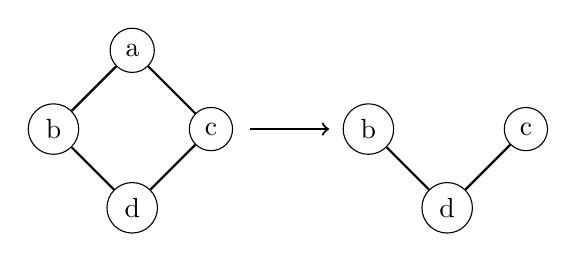
\begin{tikzpicture}
        \node[circle, draw] (a) at (2, 1) {a};
        \node[circle, draw] (b) at (1, 0) {b};
        \node[circle, draw] (c) at (3, 0) {c};
        \node[circle, draw] (d) at (2, -1) {d};
        
        \draw[thick] (a) -- (b);
        \draw[thick] (a) -- (c);
        \draw[thick] (b) -- (d);
        \draw[thick] (c) -- (d);

        \draw[->, thick] (3.5, 0) -- (4.5, 0);

        \node[circle, draw] (b1) at (5, 0) {b};
        \node[circle, draw] (c1) at (7, 0) {c};
        \node[circle, draw] (d1) at (6, -1) {d};

        \draw[thick] (b1) -- (d1);
        \draw[thick] (c1) -- (d1);
    \end{tikzpicture}
\end{figure} % Нужна ли эта картинка

Еще один пример неэффективной работы алгоритма Чайтина — это алгоритм SVD разложения.
В данном алгоритме используются несколько глобальных переменных и вложенных циклов.
Проблема распределения регистров возникает именно из-за глобальных переменных.  
Однако, поскольку стоимость выгрузки глобальных переменных слишком велика, в первую очередь выгружаются переменные циклов.
Это не решает проблему, так как она не связана с переменными циклов. 
В результате некоторые регистры могут оставаться свободными, несмотря на то, что переменные циклов выгружаются в память,
что ещё больше снижает эффективность работы программы.

На рисунке~\ref{fig:structure} представлена приблизительная структура кода.

\begin{figure}[h]
    \centering
    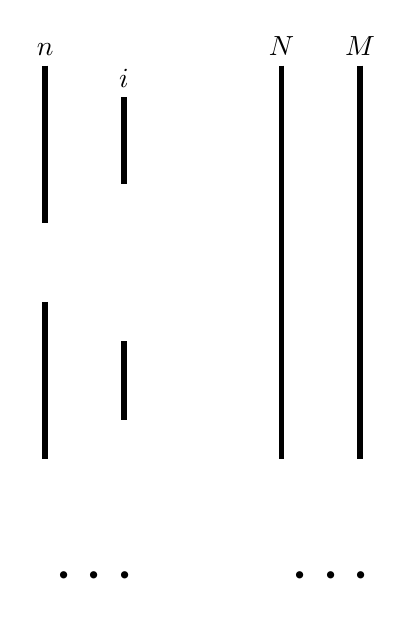
\begin{tikzpicture}
        \node[above] (n) at (0, 6) {$n$};
        \draw[line width=2pt] (n) -- (0, 4);

        \node[above] (i) at (1, 5.6) {$i$};
        \draw[line width=2pt] (i) -- (1, 4.5);

        \node[above] (N) at (3, 6) {$N$};
        \draw[line width=2pt] (N) -- (3, 1);

        \node[above] (N) at (4, 6) {$M$};
        \draw[line width=2pt] (N) -- (4, 1);

        \draw[line width=2pt] (0, 3) -- (0, 1);
        \draw[line width=2pt] (1, 2.5) -- (1, 1.5);
    
        \node at (0.625, -0.5) {\Huge $\cdots$};
        \node at (3.625,-0.5) {\Huge $\cdots$};

    \end{tikzpicture}
    \caption{Структура кода}
    \label{fig:structure}
\end{figure}

В этом коде есть переменные $i$ и $n$, это переменные циклов.
А так же есть переменные $N$ и $M$ это глобальные переменные.
Для простоты можно считать что они определяют границы циклов, при этом в самих циклах не участвуют.

\begin{figure}[H]
    \centering
    \begin{tikzpicture}
        \node[circle, draw, minimum size=1cm] (i) at (0, 0) {$i$};
        \node[circle, draw, minimum size=1cm] (n) at (0, 2) {$n$};
        \node[circle, draw, minimum size=1cm] (N) at (2, 0) {$N$};
        \node[circle, draw, minimum size=1cm] (M) at (2, 2) {$M$};
        \node[circle, draw, minimum size=1cm] (Others) at (6, 1) {\text{Другие переменные}};

        \node[below of=i] {$\frac{6}{3} = 2$};
        \node[above of=n] {$\frac{6}{3} = 2$};
        \node[below of=N] {$\frac{150}{30} = 5$};
        \node[above of=M] {$\frac{150}{30} = 5$};
        \node[above of=Others] {$\frac{100}{27} \approx 3.7$};

        \draw (i) -- (n);
        \draw (i) -- (N);
        \draw (i) -- (M);
        \draw (n) -- (N);
        \draw (n) -- (M);
        \draw (N) -- (M);

        \draw (N) -- (Others);
        \draw (M) -- (Others);
    \end{tikzpicture}
    \caption{Граф зацепленности и стоимости выгрузки}
\end{figure}

Пусть также есть другие переменные, их 27 и каждая из них имеет 100 использований.
При этом $i$ и $n$ имеют 3 соседа, и используются 6 раз.
У глобальных переменных $N$ и $M$  30 соседей, и пусть каждая из них используется 150 раз.
Будем считать что граф необходимо покрасить в 2 цвета.
Рассчитаем для каждой вершины стоимость выгрузки $\text{cost}(i) = \text{cost}(n) = \frac{6}{3} = 2$, $\text{cost}(N) = \text{cost}(M) = \frac{150}{30} = 5$,
$\text{cost}(\text{other}) = \frac{100}{27} \approx 3.7$.
Как видно в первую очередь будет производиться выгрузка переменных $i$ или $n$.

\begin{figure}[H]
    \centering
    \begin{tikzpicture}
        \node[circle, draw, minimum size=1cm] (n) at (0, 2) {$n$};
        \node[circle, draw, minimum size=1cm] (N) at (2, 0) {$N$};
        \node[circle, draw, minimum size=1cm] (M) at (2, 2) {$M$};
        \node[circle, draw, minimum size=1cm] (Others) at (6, 1) {\text{Другие переменные}};
        
        \node[above of=n] {$\frac{6}{2} = 3$};
        \node[below of=N] {$\frac{150}{29} = 5.17$};
        \node[above of=M] {$\frac{150}{29} = 5.17$};
        \node[above of=Others] {$\frac{100}{27} \approx 3.7$};

        \draw (n) -- (N);
        \draw (n) -- (M);
        \draw (N) -- (M);

        \draw (N) -- (Others);
        \draw (M) -- (Others);
    \end{tikzpicture}
    \caption{Пересчитанные стоимости}
    \label{fig:chatin_problem_2}
\end{figure}

Пересчитаем значение стоимости выгрузки (см. Рисунок~\ref{fig:chatin_problem_2}). И снова алгоритм предлагает
выгрузить переменную $n$, переменную цикла, однако это не решит проблему.
В конце переменные $M$ и $N$ будут выгружены, как и переменные $i$ и $n$.
А так как переменные $i$ и $n$ используются в цикле, то их придется очень часто выгружать и загружать, что
значительно повлияет на производительность.
